\def\ccTagRmEigenClassName{\ccFalse}
\def\ccLongParamLayout{\ccTrue}

\ccSetThreeColumns{Oriented_side}{}{\hspace*{10cm}}
\ccThreeToTwo

\chapter{dD Search Structures} 
\label{Trees}

%\ccChapterSubTitle{\rangetreeRevision, \rangetreeDate}

\minitoc

\section{Introduction}

This chapter presents the {\cgal} range tree, segment tree, and $Kd$-tree 
data structures. 
The range tree is theoretically superior to the $Kd$-tree, but the 
latter often seems to perform better.
However, the range tree as implemented in {\cgal} is more flexible than the
$Kd$-tree implementation, in that it enables to layer together range trees 
and segment trees in the same data structure.

\section{Definitions}
This section presents $d$-dimensional range and segment trees.
A one-dimensional range tree is a binary search tree on 
{\em{one-dimensional point data}}. 
Here we call all one-dimensional data types having a strict ordering
(like integer and double) {\em point data}. 
{\em{$d$-dimensional point data}} are $d$-tuples of one-dimensional 
point data.

A one-dimensional segment tree is a binary search tree as well, but with
{\em{one-dimensional interval data}} as input data.
One-dimensional interval data is a pair (i.e., 2-tuple) $(a,b)$, where $a$ 
and $b$ are one-dimensional point data of the same type and $a< b$. 
The pair $(a,b)$ represents a half open interval $[a,b)$.
Analogously, a $d$-dimensional interval  is represented by a $d$-tuple of
one-dimensional intervals.

The {\em{input data type}} for a $d$-dimensional tree is a container 
class consisting of a $d$-dimensional point data type, interval data type 
or a mixture of both, and optionally a {\em{value type}}, which 
can be used to store arbitrary data. 
E.g., the $d$--dimensional bounding box of a $d$--dimensional polygon 
may define the interval data of a $d$--dimensional segment tree and
the polygon itself can be stored as its value.   
An {\em{input data item}} is an instance of an input data type.

The range and segment tree classes are fully generic in the sense that they 
can be used to define {\em{multilayer trees}}. 
A multilayer tree of dimension (number of layers) $d$ is a simple tree in 
the $d$-th layer, whereas the $k$-th layer, $1\leq k\leq d-1$, of the tree 
defines a tree where each (inner) vertex contains a multilayer tree of 
dimension $d-k+1$.
The $k-1$-dimensional tree which is nested in the $k$-dimensional tree 
($T$) is called the {\em sublayer tree} (of $T$).
For example, a $d$-dim tree can be a range tree on the first layer, 
constructed with respect to the first dimension of $d$-dimensional data 
items.
On all the data items in each subtree, a $(d-1)$-dimensional tree is built,
either a range or a segment tree, with respect to the second dimension of 
the data items.
And so on.
%E.g., for each inner vertex of a range tree, a sublayer tree is created 
%according to all data items of the subtree of that vertex. 
%For each vertex of a segment tree an instance (tree)  is created according 
%to all data items of that vertex.
%E.g., one can define a segment tree for which each vertex contains a 
%range tree.
\lcTex{
Figures~\ref{User:fig:range.eps}, \ref{User:fig:d-range.eps} and
\ref{User:fig:d-segment.eps} illustrate the meaning of a sublayer tree
graphically.
}
\lcHtml{
The figures in Sections~\ref{sec:range_trees} and~\ref{sec:segment_trees}
illustrate the means of a sublayer tree graphically.
}

After creation of the tree, further insertions or deletions of data items 
are disallowed.  
The tree class does neither depend on the type of data nor on the concrete
physical representation of the data items.
E.g., let a multilayer tree be a segment tree for which each vertex
defines a range tree. 
We can choose the data items to consist of intervals of type \ccStyle{double} 
and the point data of type \ccStyle{integer}. 
As value type we can choose  \ccStyle{string}.

For this generality we have to
define what the tree of each dimension looks like and how the
input data is organized.
For dimension $k$, $1\le k\le 4$, \cgal\/ provides ready-to-use
range and segment trees that can store k-dimensional keys
(intervals resp.). 
Examples illustrating the use of these classes are given in
Sections~\ref{sec:range_tree_ex}
and~\ref{sec:segment_tree_ex}.
The description of the functionality of these classes as well as
the definition of higher dimensional trees and mixed multilayer
trees is given in the reference manual.

In the following two sections we give short definitions of the version of
the range tree and segment tree implemented here together with some
examples. The presentation closely follows~\cite{bkos-cgaa-97}.

\section{Software Design}


\section{Range Trees}
A one-dimensional range tree is a binary search tree on one-dimensional 
point data. 
The point data of the tree is stored in the leaves. 
Each inner vertex stores the highest entry of its left subtree.
The version of a range tree implemented here is static, which means that 
after construction of the tree, no elements be inserted or deleted.
A $d$-dimensional range tree is a binary leaf search tree according to the 
first dimension of the $d$-dimensional point data, where each vertex contains 
a $(d-1)$-dimensional search tree of the points in the subtree (sublayer tree)
with respect to the second dimension.
See~\cite{bkos-cgaa-97} and~\cite{s-dasds-90} for more detailed information.

A $d$-dimensional range tree can be used to determine all
$d$-dimensional points that lie inside  a given $d$-dimensional
interval (\ccStyle{window\_query}).
\begin{ccTexOnly}
Figure~\ref{User:fig:range.eps} shows a two-dimensional range tree,
Figure~\ref{User:fig:d-range.eps} a $d$-dimensional one.
\end{ccTexOnly}
\begin{ccHtmlOnly}
The pictures below show a two-dimensional and a <MATH>d</MATH>-dimensional
range tree.
\end{ccHtmlOnly}
\begin{ccTexOnly}
    \begin{figure}[htbp]
    \begin{minipage}{7cm}
    \begin{center}
    \includegraphics[width=7cm,clip]{SearchStructures/range2.eps}
    \end{center}
    \caption{\label{User:fig:range.eps}A two-dimensional range tree. The
      tree is a binary search tree on the first dimension. Each
      sublayer tree of a vertex $v$ is a binary search tree on the second
      dimension. The data items in a sublayer tree of $v$ are
      all data items of the subtree of $v$.}
    \end{minipage}
    \hspace*{1em}
    \begin{minipage}{7cm}
    \begin{center}
    \includegraphics[width=7cm,clip]{SearchStructures/d-range.eps}
    \end{center}
    \caption{\label{User:fig:d-range.eps}A d-dimensional range tree. For
      each layer of the tree, one
      sublayer tree is illustrated.}
    \vspace{2\baselineskip}
    %
    \end{minipage}
    \end{figure}
\end{ccTexOnly}

\begin{ccHtmlOnly}
    <!2><TABLE BORDER=0 CELLSPACING=2 CELLPADDING=0 WIDTH=650>
        <TR><TD ALIGN=LEFT VALIGN=TOP WIDTH=50% NOWRAP COLSPAN=2>
    <A NAME="User:fig:range.eps"><img border=0 src="./range2.gif" alt="A two-dimensional range tree"></A>
    </TD>
    <A NAME="User:fig:d-range.eps"><TD ALIGN=LEFT VALIGN=TOP WIDTH=50%><img border=0 src="./d-range.gif" alt="A d-dimensional range tree"></A>
      </TD></TR></TABLE>
        <!2><TABLE BORDER=0 CELLSPACING=2 CELLPADDING=0 WIDTH=650>
        <TR><TD ALIGN=LEFT VALIGN=TOP WIDTH=45%  COLSPAN=2>
    A two-dimensional range tree. The
      tree is a binary search tree on the first dimension. Each
      sublayer tree of a vertex <MATH>v</MATH> is a binary search tree on the
second
      dimension. The data items in a sublayer tree of <MATH>v</MATH> are
      all data items of the subtree of <MATH>v</MATH>
 </TD><TD ALIGN=LEFT VALIGN=TOP WIDTH=50%>
A d-dimensional range tree. For
      each layer of the tree, one
      sublayer tree is illustrated.
 </TD></TR>
        </TABLE><!2>

\end{ccHtmlOnly}

%The tree can be built in  ${\cal O}(n\log^{d-1} n)$ time and
%needs  ${\cal O}(n\log^{d-1} n)$ space. The $d$-dimensional points that lie in the
%$d$-dimensional query interval can be reported in ${\cal O}(\log^dn+k)$ time,
%where $n$ is the total number of points and $k$ is the number of
%reported points. 

The tree can be built in  $O(n\log^{d-1} n)$ time and
needs  $O(n\log^{d-1} n)$ space. The $d$-dimensional points that lie in the
$d$-dimensional query interval can be reported in $O(\log^dn+k)$ time,
where $n$ is the total number of points and $k$ is the number of
reported points. 

\subsection{Example for Range Tree on Map-like Data\label{sec:range_tree_ex}}

The following example program uses the predefined \ccc{
  Range_tree_2} data structure together with the predefined traits
  class \ccc{Range_tree_map_traits_2} which has two template
  arguments specifying the
  type of the point data in each dimension
  (\ccc{CGAL::Cartesian<double>}) and the value type of the
  2-dimensional point data (\ccc{char}). Therefore the \ccc{
  Range_tree_2} is defined on 2-dimensional point data each of which is
  associated with a character.
Then, a few data items are created and put into a list. After
  that the tree is constructed according to that list, a window
  query is performed, and the query elements are given out.

\begin{verbatim}

#include <CGAL/Cartesian.h>
#include <CGAL/Range_segment_tree_traits.h>
#include <CGAL/Range_tree_k.h>

typedef CGAL::Cartesian<double> K;
typedef CGAL::Range_tree_map_traits_2<K, char> Traits;
typedef CGAL::Range_tree_2<Traits> Range_tree_2_type;

int main()
{
  typedef Traits::Key Key;                
  typedef Traits::Interval Interval;    

  std::vector<Key> InputList, OutputList;
  InputList.push_back(Key(K::Point_2(8,5.1), 'a'));
  InputList.push_back(Key(K::Point_2(1,1.1), 'b'));
  InputList.push_back(Key(K::Point_2(3,2.1), 'c'));

  Range_tree_2_type Range_tree_2(InputList.begin(),InputList.end());
  Interval win(Interval(K::Point_2(4,8.1),K::Point_2(5,8.2)));
  std::cout << "\n Window Query:\n ";
  Range_tree_2.window_query(win, std::back_inserter(OutputList));
  std::vector<Key>::iterator current=OutputList.begin();
  while(current!=OutputList.end()){
    std::cout << (*current).first.x() << "," << (*current).first.y()
         << ":" << (*current++).second << std::endl;
  }
}
\end{verbatim}



\subsection{Example for Range Tree on Set-like Data}

This example illustrates the use of the range tree on
2-dimensional point data (no value is associated to a data item).
After the definition of the tree, some input data items are
created and the tree is constructed according to the input data
items.
After that, a window query is performed and the query elements
are given to standard out.

\begin{verbatim}
#include <CGAL/Cartesian.h>
#include <CGAL/Range_segment_tree_traits.h>
#include <CGAL/Range_tree_k.h>

typedef CGAL::Cartesian<double> K;
typedef CGAL::Range_segment_tree_set_traits_2<K> Traits;
typedef CGAL::Range_tree_2<Traits> Range_tree_2_type;

int main()
{
  typedef Traits::Key Key;
  typedef Traits::Interval Interval;
  std::vector<Key> InputList, OutputList;
  std::vector<Key>::iterator first, last, current;

  InputList.push_back(Key(8,5.1));
  InputList.push_back(Key(1,1.1));
  InputList.push_back(Key(3,2.1));

  Range_tree_2_type Range_tree_2(InputList.begin(),InputList.end());

  Interval win=Interval(Key(4,8.1),Key(5,8.2));
  std::cout << std::endl << "Window Query: lower left point: (4.0,5.0),";
  std::cout << "upper right point: (8.1,8.2)" << std::endl;
  Range_tree_2.window_query(win, std::back_inserter(OutputList));
  current=OutputList.begin();
  while(current!=OutputList.end()){
    std::cout << (*current).x()<< "-" << (*current).y() << std::endl;
    current++;
  }
}
\end{verbatim}



\section{Segment Trees}
%\definition
A segment tree is a static binary search tree for a given set of
coordinates. The set of coordinates is defined by the endpoints
of the input data intervals. Any two adjacent coordinates
build an elementary interval. Every leaf corresponds to an
elementary interval.
Inner vertices
correspond to the union of the subtree intervals of the vertex.
Each vertex or leaf $v$ contains a sublayer type (or a
list, if it is one-dimensional) that will contain all intervals $I$, such that
$I$  contains the interval of vertex $v$ but not the interval
of the parent vertex of $v$.

A $d$-dimensional segment tree can be used to solve the following problems:
\begin{itemize}
\item Determine all $d$-dimensional intervals that contain a
  $d$-dimensional point. This query type is called ``inverse
  range query''.
  \item Determine all $d$-dimensional intervals that enclose a
    given $d$-dimensional interval
    (\ccStyle{enclosing\_query}).
  \item Determine all $d$-dimensional intervals that partially overlap or are
    contained in a given $d$-dimensional interval (\ccStyle{window\_query}).
\end{itemize}

\begin{ccTexOnly}
In Figure~\ref{User:fig:segment2.eps} an example of a one-dimensional segment 
tree is given. Figure~\ref{User:fig:d-segment.eps} shows a two-dimensional
segment tree.
\end{ccTexOnly}

\begin{ccHtmlOnly}
An example of a one-dimensional segment tree and an example
of a two-dimensional segment tree are shown below.
\end{ccHtmlOnly}

\begin{ccTexOnly}
\begin{figure}[htbp]
\centering
\begin{minipage}{11cm}
    \begin{center}
    \includegraphics[width=8cm,clip]{SearchStructures/segment2.eps}
    \end{center}
\caption{\label{User:fig:segment2.eps}A one-dimensional segment
  tree. The segments and the corresponding elementary intervals
  are shown below the tree. The arcs from the nodes point to
  their subsets.}
\vspace{2\baselineskip}
\end{minipage}
\hspace*{1em}
\begin{minipage}{11cm}
    \begin{center}
    \includegraphics[width=8cm,clip]{SearchStructures/d-segment.eps}
    \end{center}
\caption{\label{User:fig:d-segment.eps}A two-dimensional segment
  tree. The first layer of the tree is built according to the
  elementary intervals of the first dimension. Each
  sublayer tree of a vertex $v$ is a segment tree according to
  the  second dimension of all data items of $v$.}

\end{minipage}
\end{figure}
\end{ccTexOnly}

\begin{ccHtmlOnly}
    <!2><TABLE BORDER=0 CELLSPACING=2 CELLPADDING=0 WIDTH=650>
        <TR>
    <A NAME="User:fig:segment2.eps"></A>
    <TD ALIGN=LEFT VALIGN=TOP WIDTH=50% NOWRAP COLSPAN=2>
    <img border=0 src="./segment2.gif" alt="A one-dimensional segment
tree">
    </TD>
    <A NAME="User:fig:d-segment.eps"></A>
    <TD ALIGN=LEFT VALIGN=TOP WIDTH=50%><img border=0
src="./d-segment.gif" alt="A d-dimensional segment tree">
      </TD></TR></TABLE>

        <!2><TABLE BORDER=0 CELLSPACING=2 CELLPADDING=0 WIDTH=650>
        <TR><TD ALIGN=LEFT VALIGN=TOP WIDTH=50%  COLSPAN=2>
A one-dimensional segment
  tree. The segments and the corresponding elementary intervals
  are shown below the tree. The arcs from the nodes point to
  their subsets.
 </TD><TD ALIGN=LEFT VALIGN=TOP WIDTH=45%>
A two-dimensional segment
  tree. The first layer of the tree is built according to the
  elementary intervals of the first dimension. Each
  sublayer tree of a vertex  <MATH>v</MATH> is a segment tree according to
  the  second dimension of all data items of  <MATH>v</MATH>.
 </TD></TR>
        </TABLE><!2>
\end{ccHtmlOnly}

%The tree can be built in  ${\cal O}(n\log^{d} n)$ time and
%needs  ${\cal O}(n\log^{d} n)$ space.
%The  processing time for inverse range
%queries in an $d$-dimensional segment tree is ${\cal O}(\log^d n
%+k)$ time, where $n$ is the total number of intervals and $k$ is
%the number of reported intervals.
The tree can be built in  $O(n\log^{d} n)$ time and
needs  $O(n\log^{d} n)$ space.
The  processing time for inverse range
queries in an $d$-dimensional segment tree is $O(\log^d n
+k)$ time, where $n$ is the total number of intervals and $k$ is
the number of reported intervals.

One possible application of a two-dimensional segment tree is the
following. Given a set of convex polygons in two-dimensional
space (CGAL::Polygon\_2), we want to determine all polygons
that intersect a given rectangular query window. Therefore, we define a
two-dimensional segment tree, where the two-dimensional interval of
a data item corresponds to the  bounding box of a polygon and the
value type corresponds to the polygon itself. The segment tree is created
with a sequence of all data items, and a window query is
performed. The polygons of the resulting data items are finally
tested independently for intersections.



\subsection{Example for Segment Tree on Map-like Data\label{sec:segment_tree_ex}}

The following example program uses the predefined \ccc{
  Segment_tree_2} data structure together with the predefined traits
  class \ccc{Segment_tree_map_traits_2} which has two template arguments
  specifying the
  type of the point data in each dimension
  (\ccc{CGAL::Cartesian<double>}) and the value type of the
  2-dimensional point data (\ccc{char}). Therefore the \ccc{
  Segment_tree_2} is defined on 2-dimensional point data
  (\ccc{CGAL::Point_2<Cartesian<double> >}) each of which is
  associated with a character.
Then, a few data items are created and put into a list. After
  that the tree is constructed according to that list, a window
  query is performed, and the query elements are given out.



\begin{verbatim}
#include <CGAL/Cartesian.h>
#include <CGAL/Segment_tree_k.h>
#include <CGAL/Range_segment_tree_traits.h>

typedef CGAL::Cartesian<double> K;
typedef CGAL::Segment_tree_map_traits_2<K, char> Traits;
typedef CGAL::Segment_tree_2<Traits > Segment_tree_2_type;

int main()
{
  typedef Traits::Interval Interval;
  typedef Traits::Pure_interval Pure_interval;
  typedef Traits::Key Key;
  std::list<Interval> InputList, OutputList1, OutputList2;

  InputList.push_back(Interval(Pure_interval(Key(1,5), Key(2,7)),'a'));
  InputList.push_back(Interval(Pure_interval(Key(2,7), Key(3,8)),'b'));
  InputList.push_back(Interval(Pure_interval(Key(6,9), Key(9,13)),'c'));
  InputList.push_back(Interval(Pure_interval(Key(1,3), Key(3,9)),'d'));
 
  Segment_tree_2_type Segment_tree_2(InputList.begin(),InputList.end());

  Interval a=Interval(Pure_interval(Key(3,6), Key(7,12)),'e');
  Segment_tree_2.window_query(a,std::back_inserter(OutputList1));

  std::list<Interval>::iterator j = OutputList1.begin();
  std::cout << "\n window_query (3,6),(7,12)\n";
  while(j!=OutputList1.end()){
    std::cout << (*j).first.first.x() << "-" << (*j).first.second.x() << " " 
         << (*j).first.first.y() << "-" << (*j).first.second.y() << std::endl; 
    j++;
  }
  
  Interval b=Interval(Pure_interval(Key(6,10),Key(7,11)), 'f');
  Segment_tree_2.enclosing_query(b,std::back_inserter(OutputList2));
  j = OutputList2.begin();
  std::cout << "\n enclosing_query (6,10),(7,11)\n";
  while(j!=OutputList2.end()){
    std::cout << (*j).first.first.x() << "-" << (*j).first.second.x() << " " 
         << (*j).first.first.y() << "-" << (*j).first.second.y() << std::endl; 
    j++;
  }
  return 0; 
}

\end{verbatim}

\subsection{Example for Segment Tree on Set-like Data}

This example illustrates the use of the predefined segment tree
on 3-dimensional interval data (with no value associated). After
the definition of the traits type and tree type, some intervals
are constructed and the tree is build according to the
intervals. Then, a window query is performed and the query
elements are given out.

\begin{verbatim}
#include <CGAL/Cartesian.h>
#include <CGAL/Segment_tree_k.h>
#include <CGAL/Range_segment_tree_traits.h>

typedef CGAL::Cartesian<int> K;
typedef CGAL::Range_segment_tree_set_traits_3<K> Traits;
typedef CGAL::Segment_tree_3<Traits > Segment_tree_3_type;

int main()
{
  typedef Traits::Interval Interval;
  typedef Traits::Key Key;
  std::list<Interval> InputList, OutputList;

  InputList.push_back(Interval(Key(1,5,7), Key(2,7,9)));
  InputList.push_back(Interval(Key(2,7,6), Key(3,8,9)));
  InputList.push_back(Interval(Key(6,9,5), Key(9,13,8)));
  InputList.push_back(Interval(Key(1,3,4), Key(3,9,8)));
 
  Segment_tree_3_type Segment_tree_3(InputList.begin(),InputList.end());

  Interval a(Key(3,6,5), Key(7,12,8));
  Segment_tree_3.window_query(a,std::back_inserter(OutputList));
  std::list<Interval>::iterator j = OutputList1.begin();
  std::cout << "\n window_query (3,6,5),(7,12,8) \n";
  while(j!=OutputList.end()){
    std::cout << (*j).first.x() << "," << (*j).first.y() << ",";
    std::cout << (*j).first.z() <<", " << (*j).second.x() << ",";
    std::cout << (*j).second.y() << "," << (*j).second.z() << std::endl; 
    j++;
  }
}
\end{verbatim}


%--------------------------------------------------------
% kd-tree.tex
%    Specification of kd-tree,
%
%  by Eyal Flato, Dan Halperin, Sariel Har-Peled
%--------------------------------------------------------
% History
% Version  1.0, 26/4/97  
%    All about kd-trees.
% Adapted by Hans Tangelder using reference pages
%--------------------------------------------------------

%\documentclass[12pt]{book}
%\usepackage{epsfig,epsf}
%\usepackage{cprog}

%\pagestyle{empty}
%\textwidth 15.6cm 
%\textheight 23 cm
%\topmargin -14mm       
%\evensidemargin 3mm 
%\oddsidemargin 3mm
%\headsep 1cm
%\def\keyword#1{{\em #1\/}}

\renewcommand{\Re}{{\rm I\!\hspace{-0.025em} R}}
%\newcommand{\Section}[1]{Section~{\ref{#1}}}
%\newcommand{\Chapter}[1]{Chapter~{\ref{#1}}}
\newcommand{\new}[1]{\marginpar{\sf #1}}
\newcommand{\kdt}{kd-tree}
\newcommand{\kdts}{kd-trees}
\newcommand{\brc}[1]{\left\{ {#1} \right\}}
\def\Ipe#1{\def\IPEfile{#1}\input{#1}}

\parindent0em
\setlength{\parskip}{1ex minus 0.9ex}
\sloppy

%\begin{document}
%\tableofcontents


\clearpage

\section{Kd-Trees} 
\label{KDT_section}

%This is a simple, but nevertheless efficient, data structure for orthogonal
%range searching.  In particular, {\cgal}  {\kdt}  seems to perform better
%than the theoreticly superior range trees, as implemented in \cgal.
%See Section \ref{KDT_sec:appendix}, for comparative results. Of
%course, the {\cgal}  range-tree implementation is more flexible than the
%{\kdt}  implementation by enabling to layer together range-trees and
%segment-trees in the same data structure, see \Chapter{Range:Trees} for the 
%details.

%The implementation of the {\kdt}  is independent of the implementation of
%the rest of {\cgal}  and can be used separately from \cgal. 

%In \Section{KDT_sec:intro}, we present the {\kdt}  structure and its
%performance. \Section{KDT_sec:class:main} presents the class
%\ccStyle{Kdtree_d<I>}.

Kd-trees are implemented by
the class \ccc{Kdtree_d}, that is parameterized with a traits class defining
the interface between the class and the geometric primitives used.
For the description of the traits classes \ccc{Kd_Interface}, \ccc{Kd_Interface_2d} 
and \ccc{Kd_Interface_3d} provided by {\cgal} please refer to the reference pages.
Also refer to the reference pages, for the description of the formal requirements for a class to be 
a kd-tree traits class by the concept \ccc{Kdtree_d_traits}.
% {\cgal}  provides ready-made interface classes that are presented in
% Section~\ref{KDT_sec:def:interface}.
% The formal requirements for a class to be a {\kdt} traits class is
% described in Section~\ref{KDT_sec:def:interface}. 


% \section{Introduction}
% \label{KDT_sec:intro}

For a given set $S = \brc{ p_1, \ldots, p_n }$ on $n$ points in
$\Re^d$, it is sometimes useful to be able to answer {\em orthogonal
   range-searching} on $S$; namely, given an axis parallel query box
$B$ in $\Re^d$, one would like to ``quickly'' determine the subset of
points of $S$ lying inside $B$.




%Orthogonal range-searching is being widely used in databases,
%computational-geometry, and vision {\large \bf (references?)}. 

Several data structures were suggested for that problem. 
Foremost among those, at least theoreticly, is the range-tree data structure
with $O(n \log^{d-1} n)$ preprocessing time, $O(n\log^{d-1} n)$ space,
and $O(\log^{d} n + k)$ query time, where $k$ is the output size of
the query.
%See \Chapter{Range:Trees} for the the {\cgal}implementation of range-trees.
A theoreticaly inferior data structure is the \kdt, which offers $O(n
\log{n})$ preprocessing time, $O(n)$ space, and $O(n^{1-1/d})$ query
time. The {\kdt}  is a binary tree constructed as follows: we compute
the point $p_i$ of $S$ such that its first coordinate is the median
value among $p_1^1, \ldots, p_n^1$, where $p_i^k$ denote the $k$-th
coordinate of the $i$-th point of $S$. Let $S_1$ denote all the points
of $S$ with first coordinate smaller than $p_i$'s first coordinate, and
let $S_2 = S \setminus S_1$.  Let $T_1,T_2$ be the {\kdts}  constructed
recursively for $S_1, S_2$, respectively.  The {\kdt}  of $S$ is simply
the binary tree having $T_1$ as its left subtree and $T_2$ as its
right subtree. We apply this algorithm recursively, splitting the sets
in the $i$-level of the {\kdt}  using the median point in the $k$-th
coordinate, where $k=(i \;\;mod \;\;n) + 1$. See Figure
\ref{KDT_fig:kdtree} for an illustration.

The resulting data structure has linear size, $O(n\log{n})$
preprocessing time, and can answer a query in $O(n^{1-1/d} +k)$ time,
where $k$ is the size of the query output. See \cite{bkos-cgaa-97}.

\begin{ccTexOnly}

\begin{figure}[hb]
    \begin{center}
        \Ipe{kdtree.ipe}
    \end{center}

    \caption{The partition of a set of  points induced by a  
       {\kdt}  of the points}

    \label{KDT_fig:kdtree}
\end{figure}

\end{ccTexOnly}

\subsection{Example illustrating orthogonal range-searching}

\ccExample

This example illustrates orthogonal range-searching. 
The {\kdt} is built using 2D points from the CGAL kernel. 

\begin{verbatim}

#include <CGAL/Cartesian.h>

#include <iostream>
#include <ctime>
#include <cassert>
#include <list>

#include <CGAL/kdtree_d.h>

typedef CGAL::Cartesian<double>           K;
typedef K::Point_2                        point;
typedef CGAL::Kdtree_interface_2d<point>  kd_interface;
typedef CGAL::Kdtree_d<kd_interface>      kd_tree;
typedef kd_tree::Box                      box;
typedef std::list<point>                  points_list;

int main()
{
    CGAL::Kdtree_d<kd_interface> tree(2);
    points_list l, res;

    std::cout << "Insering evenly 81 points  in the square (0,0)-(10,10) ...\n\n";
    for (int i=1; i<10; i++)
      for (int j=1; j<10; j++)
        {
          point p(i,j);
          l.push_front(p);
        }

    // building the tree 
    tree.build( l );
       
    // checking validity
    if  ( ! tree.is_valid() )
        tree.dump();
    assert( tree.is_valid() );

    // Defining and searching the box r
    double lx,ly,rx,ry;
    std::cout << "Define your query square.\nEnter left x coordinate: " ;
    std::cin >> lx ;
    std::cout << "Enter left y coordinate: ";
    std::cin >> ly;
    std::cout << "Enter right x coordinate: " ;
    std::cin >> rx ;
    std::cout << "Enter right y coordinate: ";
    std::cin >> ry;
    std::cout << std::endl; 

    box r(point(lx,ly), point(rx,ry) ,2);

    tree.search( std::back_inserter( res ), r );
    
    std::cout << "Listing of the points in the square: \n" ;
    std::copy (res.begin(),res.end(),std::ostream_iterator<point>(std::cout," \n") );
    std::cout << std::endl;

    tree.delete_all();

    return  0;
}

\end{verbatim}


%for html
\lcHtml{\label{KDT_fig:kdtree}}
\begin{ccHtmlOnly}
<P>
<center><img border=0 src="./kdtree.gif" alt=" "><br>
The partition of a set of  points induced by a kd-tree of the points</center>
\end{ccHtmlOnly}

\section{Reference Pages for Kd-Trees}
\label{KDT_sec:RefPages}

\begin{ccRefClass}{Kdtree_d<Traits>}

\ccThree{KdtreexdxTraitsx}{}{\hspace*{7.6cm}}
\ccTwo{}{\hspace*{7.6cm}}

%\begin{ccClassTemplate}{Kdtree_d<Traits>} 
    \ccDefinition An object $T$ of the class
    \ccStyle{Kdtree_d<Traits>} is the {\kdt}  induced by a set of points
    in $d$-dimensions.

    \ccInclude{ CGAL/kdtree_d.h}

    \ccTypes
    
    \ccNestedType{Box}{represents an axis-parallel box in
       $d$-dimensions. The box might be unbounded.}
    
    \ccTypedef{typedef Traits::Point Point;}{}
    \ccTypedef{typedef list<Point>  List_points;}{}

    \ccCreation
    \ccCreationVariable{kd_tree}
    
    \ccConstructor{Kdtree_d<Traits>( int dim = 2 );}{construct an
       empty {\kdt}   of dimension \ccStyle{dim}.}

    \ccOperations
    
\ccThree{bool}{}{\hspace*{7.6cm}}

    \ccMethod{bool is_valid(bool verbose = false, int level = 0)
       const;} {perform internal consistency checks to verify the
       correctness of the \kdt}
    
    \ccMethod{void build( list<Point> &l );}{construct the 
       {\kdt}  from the points stored in \ccStyle{l}.  
       \ccPrecond{all the points in \ccStyle{l} are of dimension no
          smaller than the dimension of {{\ccVar} } itself.} }
    
    \ccMethod{void search( back_insert_iterator<List_points>
       result, Box & query_box );}{return into \ccStyle{result} all
       the points of the {{\kdt}  } that lie inside \ccStyle{query_box}}
%\end{ccClassTemplate}

\end{ccRefClass}

%\ccHeading{\ccStyle{Kdtree_d<Traits>::Box}}

%\begin{ccClassTemplate}{Kdtree_d<I>::Box} 
\begin{ccRefClass}[Kdtree_d<Traits>::]{Box} 
    \ccDefinition An object $B$ of the class
    \ccStyle{Box} is a $d$-dimensional box (it may
    be unbounded). A $d$-dimensional box is the set defined by the
    Cartesian set $[l_1, r_1) \times [l_2, r_2) \times \cdots \times
    [l_d,r_d)$.

    \ccCreation
    \ccCreationVariable{box}
    
    \ccConstructor{Box( int d );}{Construct a box corresponding to
       the whole $d$-dimensional space}
    
    \ccConstructor{Box( Point left, Right right, int d );}{ Construct
       the axis parallel box in the $d$-dimensional space defined by
       the points \ccStyle{left}, \ccStyle{right}.}

    \ccOperations
    
    \ccMethod{void set_coord_left( int k, Point & left );}{ set
       the left endpoint of the $k$-th dimensional interval of \ccVar\ {}
       to be the $k$-th coordinate of \ccStyle{left}}
   
    \ccMethod{void set_coord_right( int k, Point & right );}{ set
       the right endpoint of the $k$-th dimensional interval of \ccVar\ {}
       to be the $k$-th coordinate of \ccStyle{right}}
    
    \ccMethod{bool is_in( Point pnt );}{return \ccStyle{true}
       if \ccStyle{pnt} lies inside \ccVar.}
    
    \ccMethod{bool is_coord_in_range( int k, Point pnt );}{ return
       \ccStyle{true} if the $k$-th coordinate of \ccStyle{pnt} lies
       inside the $k$-th dimensional interval of \ccVar.}
%\end{ccClassTemplate}
%\end{ccClass}
\end{ccRefClass}

%********************************************************
\begin{ccRefConcept}{Kdtree_d_traits}

The \ccStyle{Kdtree_d}  class is  parameterized with the
interface class \ccStyle{Traits} which defines the abstract interface
between the \ccStyle{Kdtree_d} class and the data (i.e., points). The following
requirement catalog lists the primitives, i.e.,~types, member functions
etc., that must be defined for a class that can be used to
parameterize \kdts. Ready-made implementation are available
by the \ccStyle{Kdtree_d} default traits classes.

\ccThree{static void}{}{\hspace*{7.1cm}}
\ccTwo{}{\hspace*{7.1cm}}


\begin{ccClass} {Traits}

    \ccCreationVariable{t}

    \ccDefinition
    A class \ccClassName\ that satisfies the requirements of an
    interface class for a \ccStyle{Kdtree_d} class must provide the
    following types and operations. 
  
    \ccTypes
    
    \ccNestedType{Point}{A type to hold a input item.}

    \ccOperations
%    \ccSetTwoOfThreeColumns{4cm}{4cm}

    \ccMethod{static Comparison_result compare(
       int k,
       const Point & p0,
       const Point & p1);} {compare the \ccStyle{k}-th coordinate
       of $p0$ and $p1$.  Return \ccStyle{LARGER} if $p0_k >
       p1_k$, \ccStyle{SMALLER} if $p0_k < p1_k$, or else
       \ccStyle{EQUAL}.  }

    \ccMethod{static void  copy_coord( int  k, Point   & dest, 
       const Point & src );}{Copy the $k$-th coordinate of $src$ to
       the $k$-th coordinate of $dest$.}

    \ccMethod{static int  dimension( const Point  & pnt );}
    {return the dimension of \ccStyle{pnt}}
\end{ccClass}
\end{ccRefConcept}

\begin{ccRefClass}{Kdtree_Interface<Point>}

{\cgal}  contains a default implementation for the Kdtree\_d traits
class, that
may be applied to any
standard class of point provided by \cgal.

The default traits class \ccStyle{Kdtree_Interface<Point>} is
templated with a parameter \ccStyle{Point}, which is required to
supply the following methods:

\begin{itemize}
    \item Constructor, and copy constructor.

    \item \ccStyle{int dimension();} - return the dimension of the point.
    
    \item \ccStyle{operator[](int dim);} - an operator for accessing
    the various coordinates of the given point. Used also to copy
    coordinates between points.
\end{itemize}

There are two other default traits classes \ccStyle{Kdtree_Interface_2d<Point>} 
and \ccStyle{Kdtree_Interface_3d<Point>} which should be used when using 
2D and 3D points from the {\cgal} kernel. This is done since the points in the
kernel do not support changing their coordinates through direct access. 

\end{ccRefClass}
%********************************************************

%********************************************************
\begin{ccRefClass}{Kdtree_Interface_2d<Point>}

The default traits class \ccStyle{Kdtree_Interface_2d<Point>} 
should be used when using 2D points from the {\cgal} kernel.
It is
templated with a parameter \ccStyle{Point}, which is required to
supply the following methods:

\begin{itemize}
    \item Constructor, and copy constructor.

    \item \ccStyle{int dimension();} - return the dimension of the point.
    
    \item \ccStyle{operator[](int dim);} - an operator for accessing
    the various coordinates of the given point. Used also to copy
    coordinates between points.
\end{itemize}

\end{ccRefClass}

%********************************************************
\begin{ccRefClass}{Kdtree_Interface_3d<Point>}

The default traits class \ccStyle{Kdtree_Interface_3d<Point>} 
should be used when using 3D points from the {\cgal} kernel.
It is
templated with a parameter \ccStyle{Point}, which is required to
supply the following methods:

\begin{itemize}
    \item Constructor, and copy constructor.

    \item \ccStyle{int dimension();} - return the dimension of the point.
    
    \item \ccStyle{operator[](int dim);} - an operator for accessing
    the various coordinates of the given point. Used also to copy
    coordinates between points.
\end{itemize}

\end{ccRefClass}

%*********************************************************

%-------------------------------------------------------------------------
% Bibiliography 
%-------------------------------------------------------------------------

%\bibliographystyle{alpha}
%\bibliography{geometry}


%\end{document}

%%% Local Variables: 
%%% mode: latex
%%% TeX-master: t
%%% End: 




